\documentclass[border=4pt]{standalone}

\usepackage{pgfplots}
\usepackage{pgfplotstable}
\pgfplotsset{compat=1.18, width=8.5cm, height=5.6cm, tick label style={font=\small}, label style={font=\small}, legend cell align=left, legend style={font=\small, draw=none, fill=none}}

\definecolor{plnavy}{HTML}{1F4E89}
\definecolor{plrose}{HTML}{B85A52}
\definecolor{plsage}{HTML}{93CC9E}
\definecolor{plsand}{HTML}{E0BE78}
\definecolor{plplum}{HTML}{8E7BB5}
\definecolor{plgray}{HTML}{6E6E6E}

% ==== data: \ridge{row}{center}{width}{color}, last row first so nearer curves overlap ====
\newcommand{\ridges}{
  \ridge{4}{2.0}{0.70}{plgray}
  \ridge{3}{3.1}{0.80}{plrose}
  \ridge{2}{4.0}{0.65}{plsand}
  \ridge{1}{5.2}{0.75}{plsage}
  \ridge{0}{6.3}{0.60}{plnavy}
}
\pgfplotsset{row names/.style={ytick={0,1,2,3,4}, yticklabels={Epoch 100,Epoch 75,Epoch 50,Epoch 25,Epoch 1}}}

\newcommand{\ridge}[4]{
  \addplot[fill=#4!45, draw=#4!80!black, thick, domain=0:9, samples=121] {#1+1.5*exp(-0.5*((x-#2)/#3)^2)} -- (axis cs:9,#1) -- (axis cs:0,#1) -- cycle;
}

\begin{document}
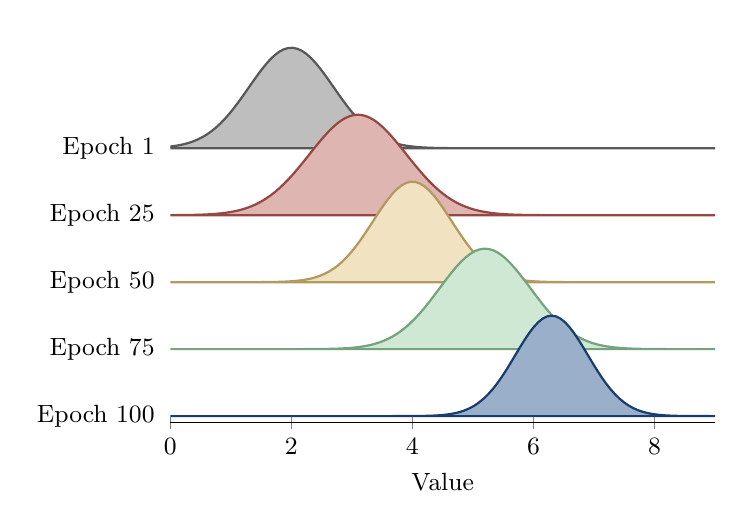
\begin{tikzpicture}
\begin{axis}[height=6.6cm, xmin=0, xmax=9, ymin=-0.1, ymax=5.8, axis lines=left, axis line style={-}, y axis line style={draw=none}, ytick style={draw=none}, row names, xlabel={Value}]
  \ridges
\end{axis}
\end{tikzpicture}
\end{document}
